%\{Параметры перенацеливания}
Максимальный диапазон углового перенацеливания камеры:
$\beta_{max} = -45..+45^{\circ}$
Привод должен обеспечивать режимы переброски удовлетворяющие следующим 3м движениям:

\begin{enumerate}
    \item Перенацеливание камеры на $q = 20^{\circ}$ за $t_{\text{п}} = 2   \text{с}$
    \item Перенацеливание камеры на $q = 45^{\circ}$ за $t_{\text{п}} = 3   \text{с}$
    \item Перенацеливание камеры на $q = 90^{\circ}$ за $t_{\text{п}} = 4.3 \text{с}$
\end{enumerate}

Пусть $t_\text{п}$ – время перенацеливания камеры из точки $\beta_{H}$ в точку $\beta_{K}$.
Заданная траектория движения камеры $\beta(t)$ (зависимость вращения камеры от времени)
будет заранее рассчитываться (планироваться) как плавная симметричная
(относительно точки $\frac{t_\text{п} }{2}$) траектория.
Соответственно, заданная траектория движения нагрузки $q_{i}(t)$
(зависимость вращения нагрузки от времени) каждого из двух приводов будет рассчитываться
(планироваться) как плавная симметричная (относительно точки $\frac{t_\text{п} }{2}$)
траектория, которую приводной блок должен отследить с заданной точностью.
Т.е. система управления приводом должна воспроизводить заданный закон изменения управляющего
воздействия.
Симметричная (относительно точки $\frac{t_\text{п} }{2}$) траектория будет представлять
собой разгон камеры (нагрузки) на отрезке времени от 0 до $\frac{t_\text{п} }{2}$
и замедление на отрезке времени от $\frac{t_\text{п} }{2}$ до $t_\text{п}$.

Будем полагать, что большинство траекторий перенацеливания камеры могут быть заданы
в виде эквивалентного входного гармонического сигнала
(рис. \ref{retarget_20grad_2sec},
      \ref{retarget_45grad_3sec},
      \ref{retarget_90grad_4,3sec}).
Определим параметры типовых траекторий перенацеливания с помощью следующих формул:

\begin{equation}
    \label{retarget_angle}
    \omega_{\beta.p} \cdot \frac{t_\text{п} }{2} = \frac{\pi}{2}
\end{equation}

\begin{equation}
    \label{equiv_signal_frequency}
    \omega_{\beta.p} = \frac{\pi}{t_\text{п} } ~c^{-1}
\end{equation}

\begin{equation}
    \label{max_speed_for_equiv_signal}
    \dot{\beta}_{max} = A_\text{экв} \cdot \omega_{\beta.p} ~\text{град}^{\circ} / c
\end{equation}

\begin{equation}
    \label{max_acceleration_for_equiv_signal}
    \ddot{\beta}_{max} = \dot{\beta}_{max} \cdot \omega_{\beta.p} ~\text{град}^{\circ} / c^{2}
\end{equation}

где $\omega_{\beta.p}$ - рабочая частота эквивалентного гармонического сигнала,

$\dot{\beta}_{max}$ - максимальная угловая скорость вращения камеры,
соответствующая параметрам эквивалентной синусоиды

$\ddot{\beta}_{max}$ - максимальное ускорение вращения камеры,
соответствующее параметрам эквивалентной синусоиды

$A_\text{экв}$ – амплитуда эквивалентного гармонического сигнала

\subsubsection{Перенацеливание, режим 1}

\textbf{Параметры: $q = 20^{\circ}$ за $t_{\text{п}} = 2$ c}

Представим данный участок (от $\beta_{H}$ до $\beta_{K}$) в виде синусоиды
от точки $-A_\text{экв}$ до точки $+A_\text{экв}$ на участке полупериода
(рис. \ref{retarget_20grad_2sec}), $A_\text{экв}$ в данном случае
равна $\frac{q}{2} = 10^{\circ}$.

\begin{figure}[ht!]
    \centering
    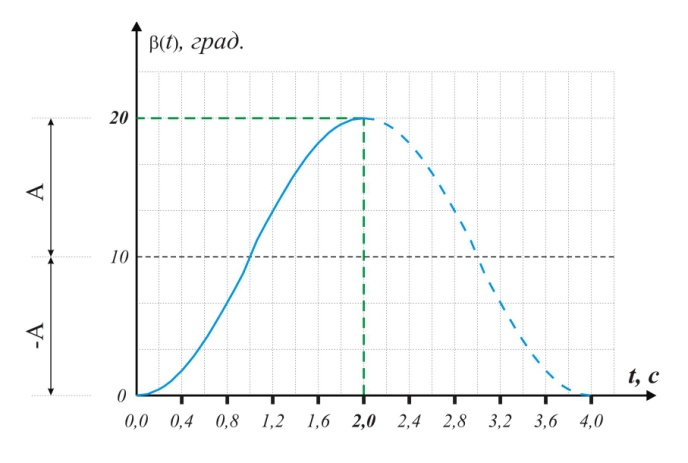
\includegraphics[keepaspectratio]{./src/pictures/retarget_equivalent_input_signals/20grad_2sec}
    \caption{Перенацеливание камеры на $q = 20^{\circ}$ за $t_\text{п} = 2$ c}
    \label{retarget_20grad_2sec}
\end{figure}

Зная $t_{\text{п} } = 2$ c, можем определить нужные нам параметры перенацеливания
с помощью (\ref{equiv_signal_frequency}),
(\ref{max_speed_for_equiv_signal}),
(\ref{max_acceleration_for_equiv_signal}):

$$
    \omega_{\beta.p} = \frac{\pi}{2} = 1.57 ~c^{-1}
$$
$$
    \dot{\beta}_{max} = 10 \cdot 1.57 = 15.7 ~\text{град}^{\circ} / c
$$
$$
    \ddot{\beta}_{max} = 15.7 \cdot 1.57 = 24.65 ~\text{град}^{\circ} / c^{2}
$$

%\subsubsection{Перенацеливание камеры на $q = 45^{\circ}$ за $t_{\text{п}} = 3$ c}
\subsubsection{Перенацеливание, режим 2}

\textbf{Параметры: $q = 45^{\circ}$ за $t_{\text{п}} = 3$ c}

Представим данный участок (от $\beta_{H}$ до $\beta_{K}$) в виде синусоиды от
точки $-A_\text{экв}$ до точки $+A_\text{экв}$ на участке полупериода
(рис. \ref{retarget_45grad_3sec}), $A_\text{экв}$ в данном случае равна
$\frac{q}{2} = 22.5^{\circ}$.

\begin{figure}[h!]
    \centering
    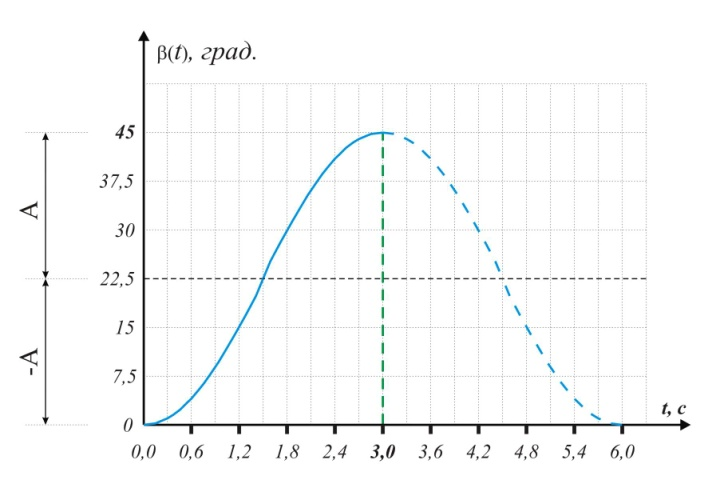
\includegraphics[keepaspectratio]{./src/pictures/retarget_equivalent_input_signals/45grad_3sec}
    \caption{Перенацеливание камеры на $q = 45^{\circ}$ за $t_\text{п} = 3$ c}
    \label{retarget_45grad_3sec}
\end{figure}

Зная $t_{\text{п} } = 3$ c, можем определить нужные нам параметры перенацеливания
с помощью (\ref{equiv_signal_frequency}),
(\ref{max_speed_for_equiv_signal}),
(\ref{max_acceleration_for_equiv_signal}):

$$
    \omega_{\beta.p} = \frac{\pi}{3} = 1.047 ~c^{-1}
$$
$$
    \dot{\beta}_{max} = 22.5 \cdot 1.047 = 23.56 ~\text{град}^{\circ} / \text{с}
$$

$$
    \ddot{\beta}_{max} = 23.56 \cdot 1.047 = 24.67 ~\text{град}^{\circ} / \text{с}^{2}
$$

%\subsubsection{Перенацеливание камеры на $q = 90^{\circ}$ за $t_\text{п} = 4.3$ c}
\subsubsection{Перенацеливание, режим 3}

\textbf{Параметры: $q = 90^{\circ}$ за $t_\text{п} = 4.3$ c}

Представим данный участок (от $\beta_{H}$ до $\beta_{K}$) в виде синусоиды от точки
$-A_\text{экв}$ до точки $+A_\text{экв}$ на участке полупериода
(рис. \ref{retarget_90grad_4,3sec}), $A_\text{экв}$ в данном случае
равна $\frac{q}{2} = 45^{\circ}$.

\begin{figure}[ht!]
    \centering
    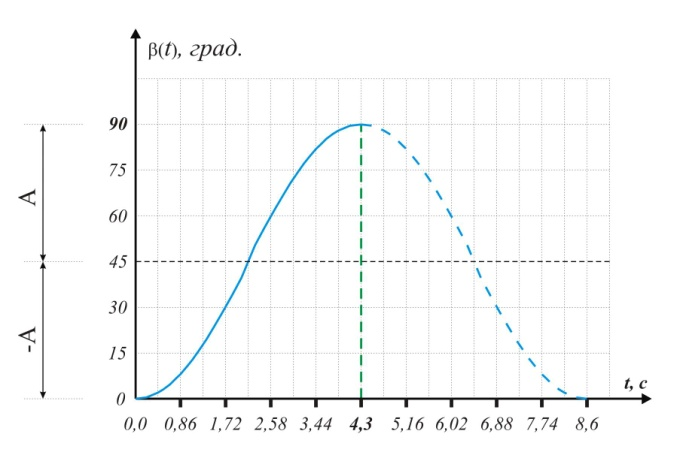
\includegraphics[keepaspectratio]{./src/pictures/retarget_equivalent_input_signals/90grad_4,3sec}
    \caption{Перенацеливание камеры на $q = 90^{\circ}$ за $t_\text{п} = 4.3$ c}
    \label{retarget_90grad_4,3sec}
\end{figure}

Зная $t_{\text{п} } = 4.3$ c, можем определить нужные нам параметры перенацеливания
с помощью (\ref{equiv_signal_frequency}),
(\ref{max_speed_for_equiv_signal}),
(\ref{max_acceleration_for_equiv_signal}):

$$
    \omega_{\beta.p} = \frac{\pi}{4.3} = 0.73 ~c^{-1}
$$
$$
    \dot{\beta}_{max} = 45 \cdot 0.73 = 32.85 ~\text{град}^{\circ} / c
$$
$$
    \ddot{\beta}_{max} = 32.85 \cdot 0.73 = 23.98 ~\text{град}^{\circ} / c^{2}
$$

\endinput

